\documentclass[11pt,compress,t,notes=noshow, aspectratio=169, xcolor=table]{beamer}

\usepackage{../../style/lmu-lecture}
% Defines macros and environments
% This file is included in slides and exercises

% Rarely used fontstyle for R packages, used only in 
% - forests/slides-forests-benchmark.tex
% - exercises/single-exercises/methods_l_1.Rnw
% - slides/cart/attic/slides_extra_trees.Rnw
\newcommand{\pkg}[1]{{\fontseries{b}\selectfont #1}}

% Spacing helpers, used often (mostly in exercises for \dlz)
\newcommand{\lz}{\vspace{0.5cm}} % vertical space (used often in slides)
\newcommand{\dlz}{\vspace{1cm}}  % double vertical space (used often in exercises, never in slides)
\newcommand{\oneliner}[1] % Oneliner for important statements, used e.g. in iml, algods
{\begin{block}{}\begin{center}\begin{Large}#1\end{Large}\end{center}\end{block}}

% Don't know if this is used or needed, remove?
% textcolor that works in mathmode
% https://tex.stackexchange.com/a/261480
% Used e.g. in forests/slides-forests-bagging.tex
% [...] \textcolor{blue}{\tfrac{1}{M}\sum^M_{m} [...]
% \makeatletter
% \renewcommand*{\@textcolor}[3]{%
%   \protect\leavevmode
%   \begingroup
%     \color#1{#2}#3%
%   \endgroup
% }
% \makeatother


\title{Interpretable Machine Learning}
% \author{LMU}
%\institute{\href{https://compstat-lmu.github.io/lecture_iml/}{compstat-lmu.github.io/lecture\_iml}}
\date{}

\begin{document}

\newcommand{\titlefigure}{figure/whitebox}
\newcommand{\learninggoals}{
\item What characteristics does an interpretable model have?
\item Why should we use interpretable models at all?
\item Examples for interpretable models.}

\lecturechapter{Interpretable Models}
\lecture{Interpretable Machine Learning}

\begin{frame}{Motivation}

    \begin{itemize}
        %\item Obtaining interpretations by using interpretable models is the easiest and least error-prone approach.
        \item Achieving interpretability by using interpretable models is the most straightforward approach.
        \bigskip
        \item Classes of models deemed interpretable:
        \begin{itemize}
            %\item Linear regression models
            \item (Generalized) linear models
            \item Generalized additive models
            \item Rule-based learning
            \item Model-based boosting / component-wise boosting
            \item ...
        \end{itemize}
    \end{itemize}

\end{frame}

\begin{frame}{Advantages}

    \begin{itemize}[<+->]
    \itemsep1em
        \item Additional model-agnostic interpretation techniques not required.\\
        $\Rightarrow$ Eliminates a source of error.
        \item Since interpretable models are often simple, training time is fairly small.
        \item Some interpretable models fulfill the monotonicity constraint.\\
        $\leadsto$ Larger feat. values always lead to higher (or smaller) outcomes (e.g., GLMs).
        \item Many people are familiar with traditional interpretable models.\\
        $\Rightarrow$ Increases trust in the model and facilitates communication about its results.
        \item Implementations are available in many programming languages. \\
        $\Rightarrow$ Simple models are easier to deploy in practice or implement from scratch.
    \end{itemize}

\end{frame}

\begin{frame}{Disadvantages}

    \begin{itemize}
    \itemsep1em
        \item Certain assumptions about data and / or model structure are often reqiured.\\
        $\Rightarrow$ If assumptions are wrong, models may have bad predictive performance.
        %\item If the wrong assumptions are made, interpretable models may have a bad predictive performance.
        \pause
        \item Often not able to model highly complex relationships due to limited model flexibility.
        \pause
        \item A complex structure of an interpretable model may also be difficult to interpret, e.g.:
        \begin{itemize}
            \item linear model with hundreds of features and interactions 
            \item decision trees with huge tree depth
        \end{itemize}
        \pause
        \item Still requires application of model-agnostic interpretation techniques if certain types of explanations are of interest (e.g., counterfactual explanations).
    \end{itemize}

\end{frame}

\begin{frame}{Further Comments}

    \begin{itemize}
    \itemsep1em
        \item Some argue that one should always use interpretable models in the first place \lit{Rudin 2019}{https://www.nature.com/articles/s42256-019-0048-x}
        \begin{itemize}
            \item \ldots and not try to explain uninterpretable models post-hoc.
            \item Can sometimes work out by spending enough time and energy on data pre-processing. %feat. engineering and data cleaning
        \end{itemize}
        \pause
        %\footnote[frame]{Rudin, C. Stop explaining black box machine learning models for high stakes decisions and use interpretable models instead. Nat Mach Intell 1, 206–215 (2019).}
        % {https://www.nature.com/articles/s42256-019-0048-x}
       %\item Interpretable models also have the potential for a high predictive performance, but require more knowledge and time spent on data preprocessing.
       \item[$\leadsto$] Drawback: Hard to achieve for data for which end-to-end learning is crucial\\ (e.g., images and text)
        \pause
        %\item One can assume a trade-off between interpretability and model performance which generally (but not always) holds.
        \item There might be a trade-off between interpretability and model performance (but not always).
        \pause
        \item \textbf{Recommendation:}
        \begin{itemize}
            \item Start with most simple model that makes sense for application at hand
            \item Gradually increase complexity if performance is insufficient\\
            $\leadsto$ will usually lower interpretability and require additional interpretation methods
            \item Choose the most simple, sufficient model (Occam's razor)
        \end{itemize} 
    \end{itemize}

\end{frame}



\begin{frame}{Linear and Polynomial Regression}

\begin{align*}
\mathbb{E}_Y(Y \vert X) &= \beta_0 + \beta_1 x_1 + \dots + \beta_p x_p + \dots + \epsilon \\
 &= X^T\beta + \mathcal{E}
\end{align*}

\begin{itemize}
\itemsep1em
\item Model equation is identical across the entire feature space.
%\item The predictive power of LMs is determined by specifying the correct model structure.
\item Polynomial regression extends the LM by non-linear effects and interactions.
%A polynomial regression model is an extension of the LM that includes higher order terms or interactions.
%This enables us to model non-linear data while making use of the entire arsenal of LM functionality.
\item We can exactly determine feature effects (e.g., beta coefficients, effect plots) and importance scores (e.g., p-values, t-statistics).
%By knowing the model equation, we can exactly determine feature effects (e.g., beta coefficients, effect plots) and importance scores (e.g., p-values, t-statistics).
\item For higher order effects or interactions, beta coefficients cannot be interpreted in isolation.
\item Note: For inference-based metrics (p-values, confidence intervals) to be valid, error term needs to be normally distributed with zero mean, i.e., $\epsilon \sim N(0, \sigma^2) \; \Rightarrow \; (y \vert x) \sim N(x^T \beta, \sigma^2)$.\\
$\leadsto$ Restricts use of LMs in practice as distribution of error is a prior assumption about data.
\end{itemize}
\end{frame}

\begin{frame}{Linear and Polynomial Models}

\begin{columns}[T]
\begin{column}{0.55\textwidth}
\tiny
\verbatiminput{figure/lm_output.txt}
\end{column}
\begin{column}{0.45\textwidth}  %%<--- here
  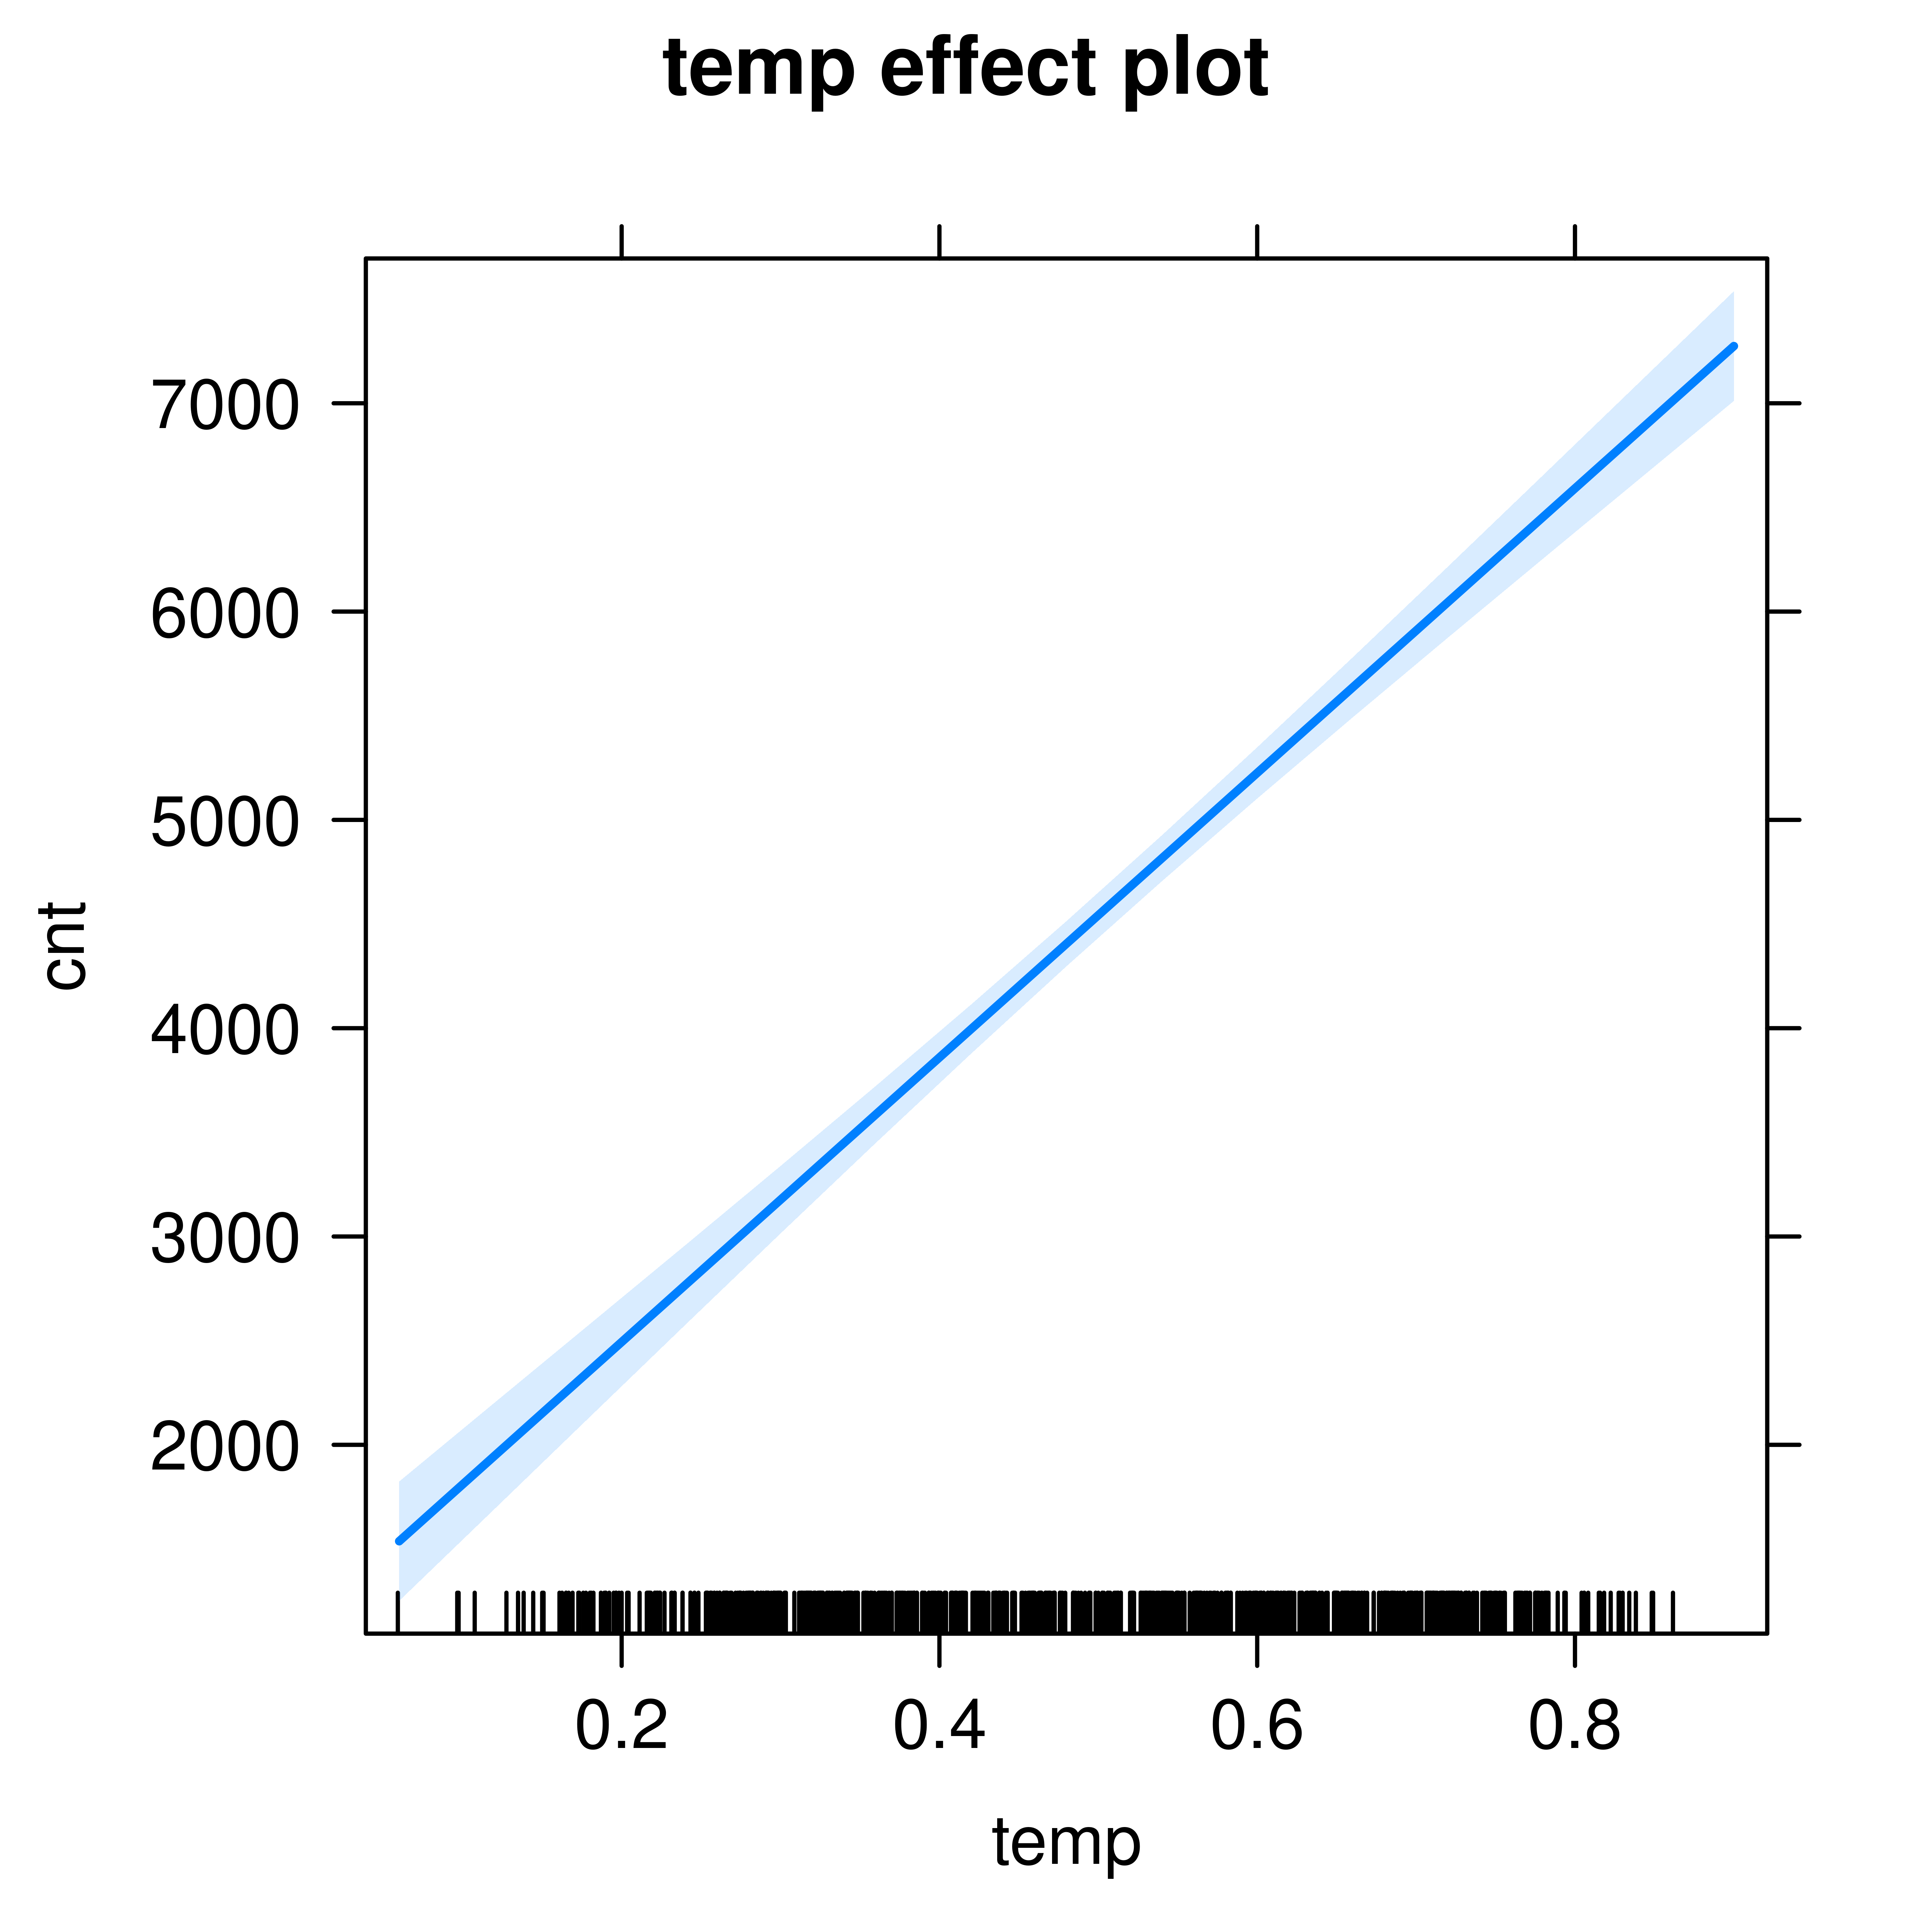
\includegraphics[width = \textwidth]{figure/lm_effect_plot.png}
\end{column}
\end{columns}
\end{frame}

\begin{frame}{Generalized Linear Models (GLMs)}

\begin{align*}
g\left(\mathbb{E}_Y(Y \vert X)\right) &= X^T\beta \\
\mathbb{E}_Y \left(Y \vert X\right) &= g^{-1}(X^T\beta)
\end{align*}
\begin{itemize}[<+->]
%\setlength\itemsep{1em}
%\item GLMs are a framework for target distributions of  exponential families (e.g., Gaussian, Binomial, Poisson, Gamma). Gaussian target distribution $+$ identity link $\hat =$ linear / polynomial model.
\item GLM framework assumes distribution of $Y$ is a member of exponential families, e.g.: % (e.g., Gaussian, Binomial, Poisson)
\begin{itemize}[<.->]
    \item Gaussian target distribution $+$ identity link $\hat =$ linear / polynomial model.
    \item Binomial target distribution $+$ logit link $log\left(\frac{\mathbb{E}_Y(Y \vert X)}{1 - \mathbb{E}_Y(Y \vert X)}\right)$ $\hat =$ logistic regression.
\end{itemize}
%\item GLMs keeps linear predictor $X^T\beta$ (explains $\mathbb{E}_Y(Y \vert X)$ through a more flexible link function $g$).
\item Link function $g$ describes how $X^T\beta$ relates to the expected, conditional target $\mathbb{E}_Y(Y \vert X)$.
\begin{itemize}[<.->]
    \item Interpretations as for linear / polynomial models but w.r.t. transformed target via $g$.
    \item Linear terms become non-linear through the link function (except for identity link)!
\end{itemize}
%\item If the target is distributed binomially, a natural link function is the logit link $log\left(\frac{\mathbb{E}_Y(Y \vert X)}{1 - \mathbb{E}_Y(Y \vert X)}\right)$ (logistic regression).
\item We need to specify the correct model equation, target distribution, and link function to receive a good model fit.
%\item %As the model equation is still known, interpretations are possible the same way as for polynomial regression models.
%However, even linear terms become non-linear through the link function (if the identity link is not used)!
\end{itemize}
\end{frame}


\begin{frame}{Generalized Linear Models}
\begin{columns}[T]
\begin{column}{0.55\textwidth}
\tiny
\verbatiminput{figure/glm_output.txt}
\end{column}
\begin{column}{0.45\textwidth}  %%<--- here
  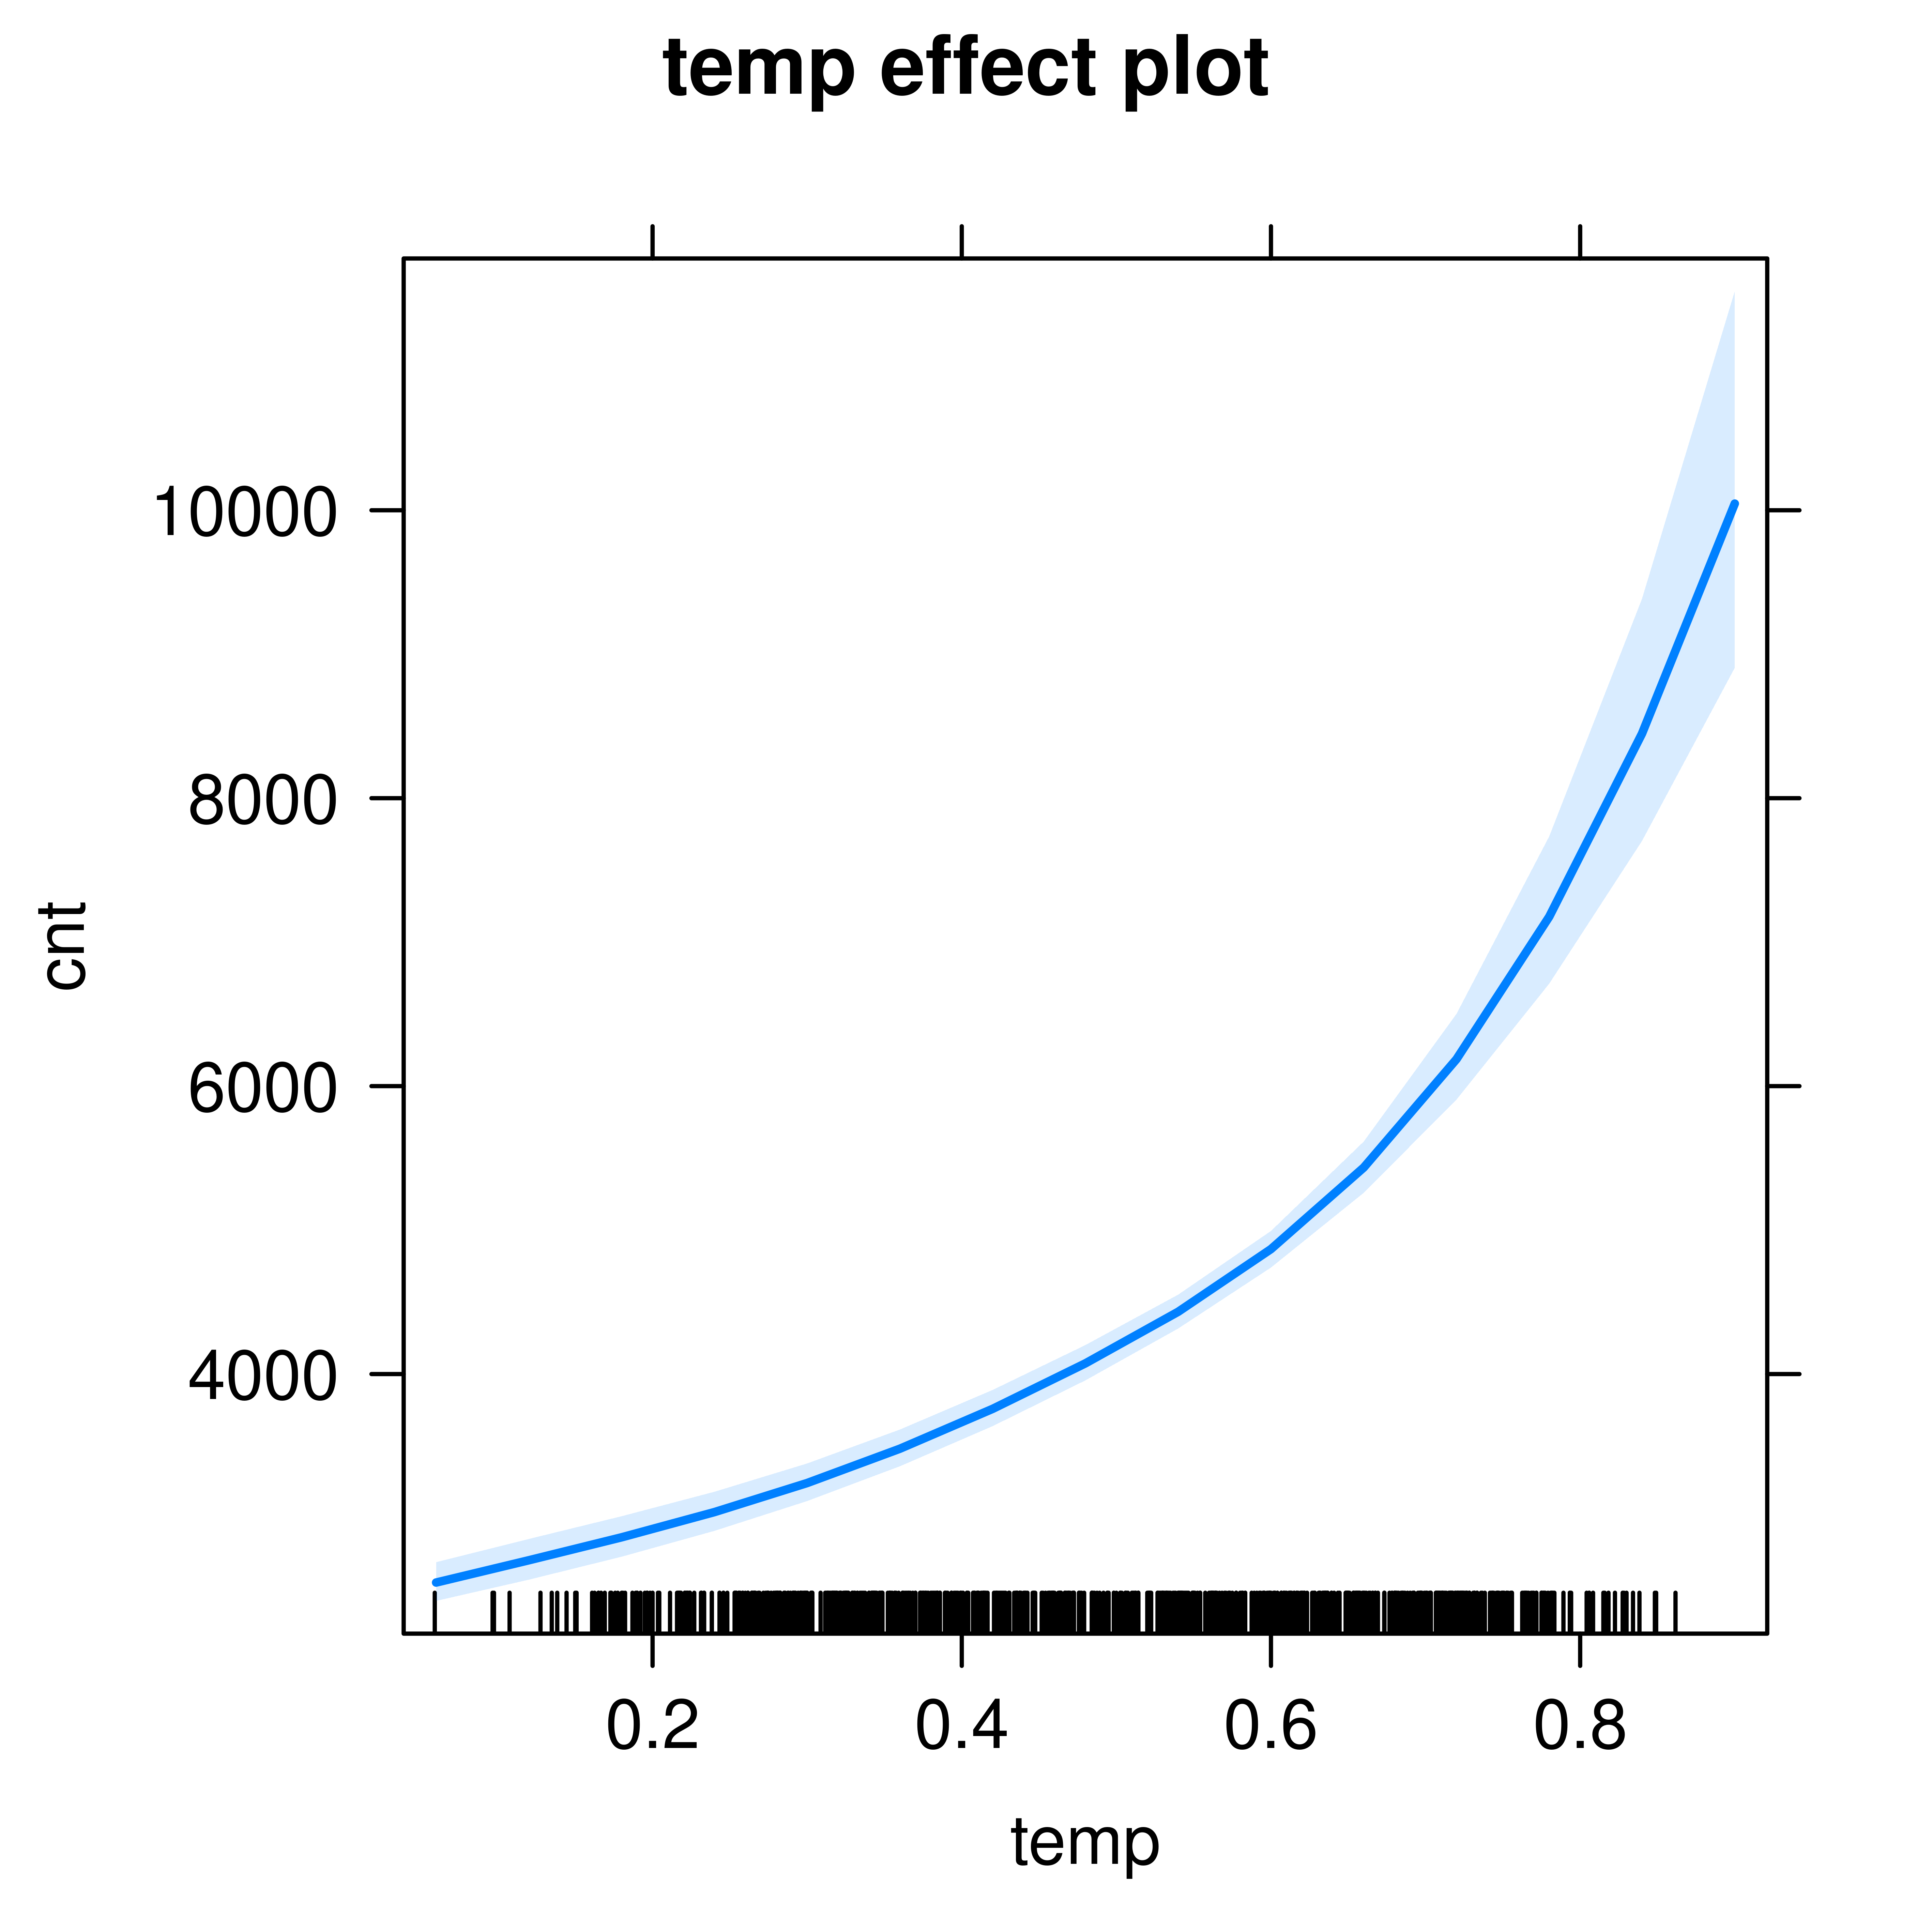
\includegraphics[width = \textwidth]{figure/glm_effect_plot.png}
\end{column}
\end{columns}
\end{frame}

\begin{frame}{Generalized Additive Models}

$$
g\left(\mathbb{E}_Y(y \vert x)\right) = \beta_0 + h_1(x_1) + \dots + h_p(x_p) + \dots
$$
\begin{itemize}
% TODO: needs to be shortened
%\setlength\itemsep{1em}
\item Replaces pre-specified linear / polynomial terms with smooth terms $h_j$.\\
$\Rightarrow h_j$ can be specified in a parametric (regression spline) or non-parametric (LOESS) way.
%\item For the component functions, we may either specify a parametric form (e.g., regression splines), or a non-parametric one, e.g., locally estimated scatterplot smoothing (LOESS).
%\item GAMs are more adaptive than GLMs as they rely more on data structure instead of pre-specified linear / polynomial terms. %prior assumptions.
%\item We still need to specify the order and type of the component functions to be estimated, e.g., which interactions to include.
\item Specification of order/type of smooth terms still required, e.g., which interactions.
%\item The smoothing degree of each component function can be tuned to avoid overfitting. Regularization increases interpretability, as the interpretations drawn from the model can be transferred more easily to new data.
\item Retains interpretability via additive model equation (if smooth terms are interpretable).
%\item
%As the model equation is known, we can use similar interpretation methods as for LMs and GLMs, e.g., evaluating the estimated components that depend on the features of interest.
\end{itemize}
\end{frame}


\begin{frame}{Generalized Additive Models}
\begin{columns}[T]
\begin{column}{0.55\textwidth}
\tiny
\verbatiminput{figure/gam_output.txt}
\end{column}
\begin{column}{0.45\textwidth}  %%<--- here
  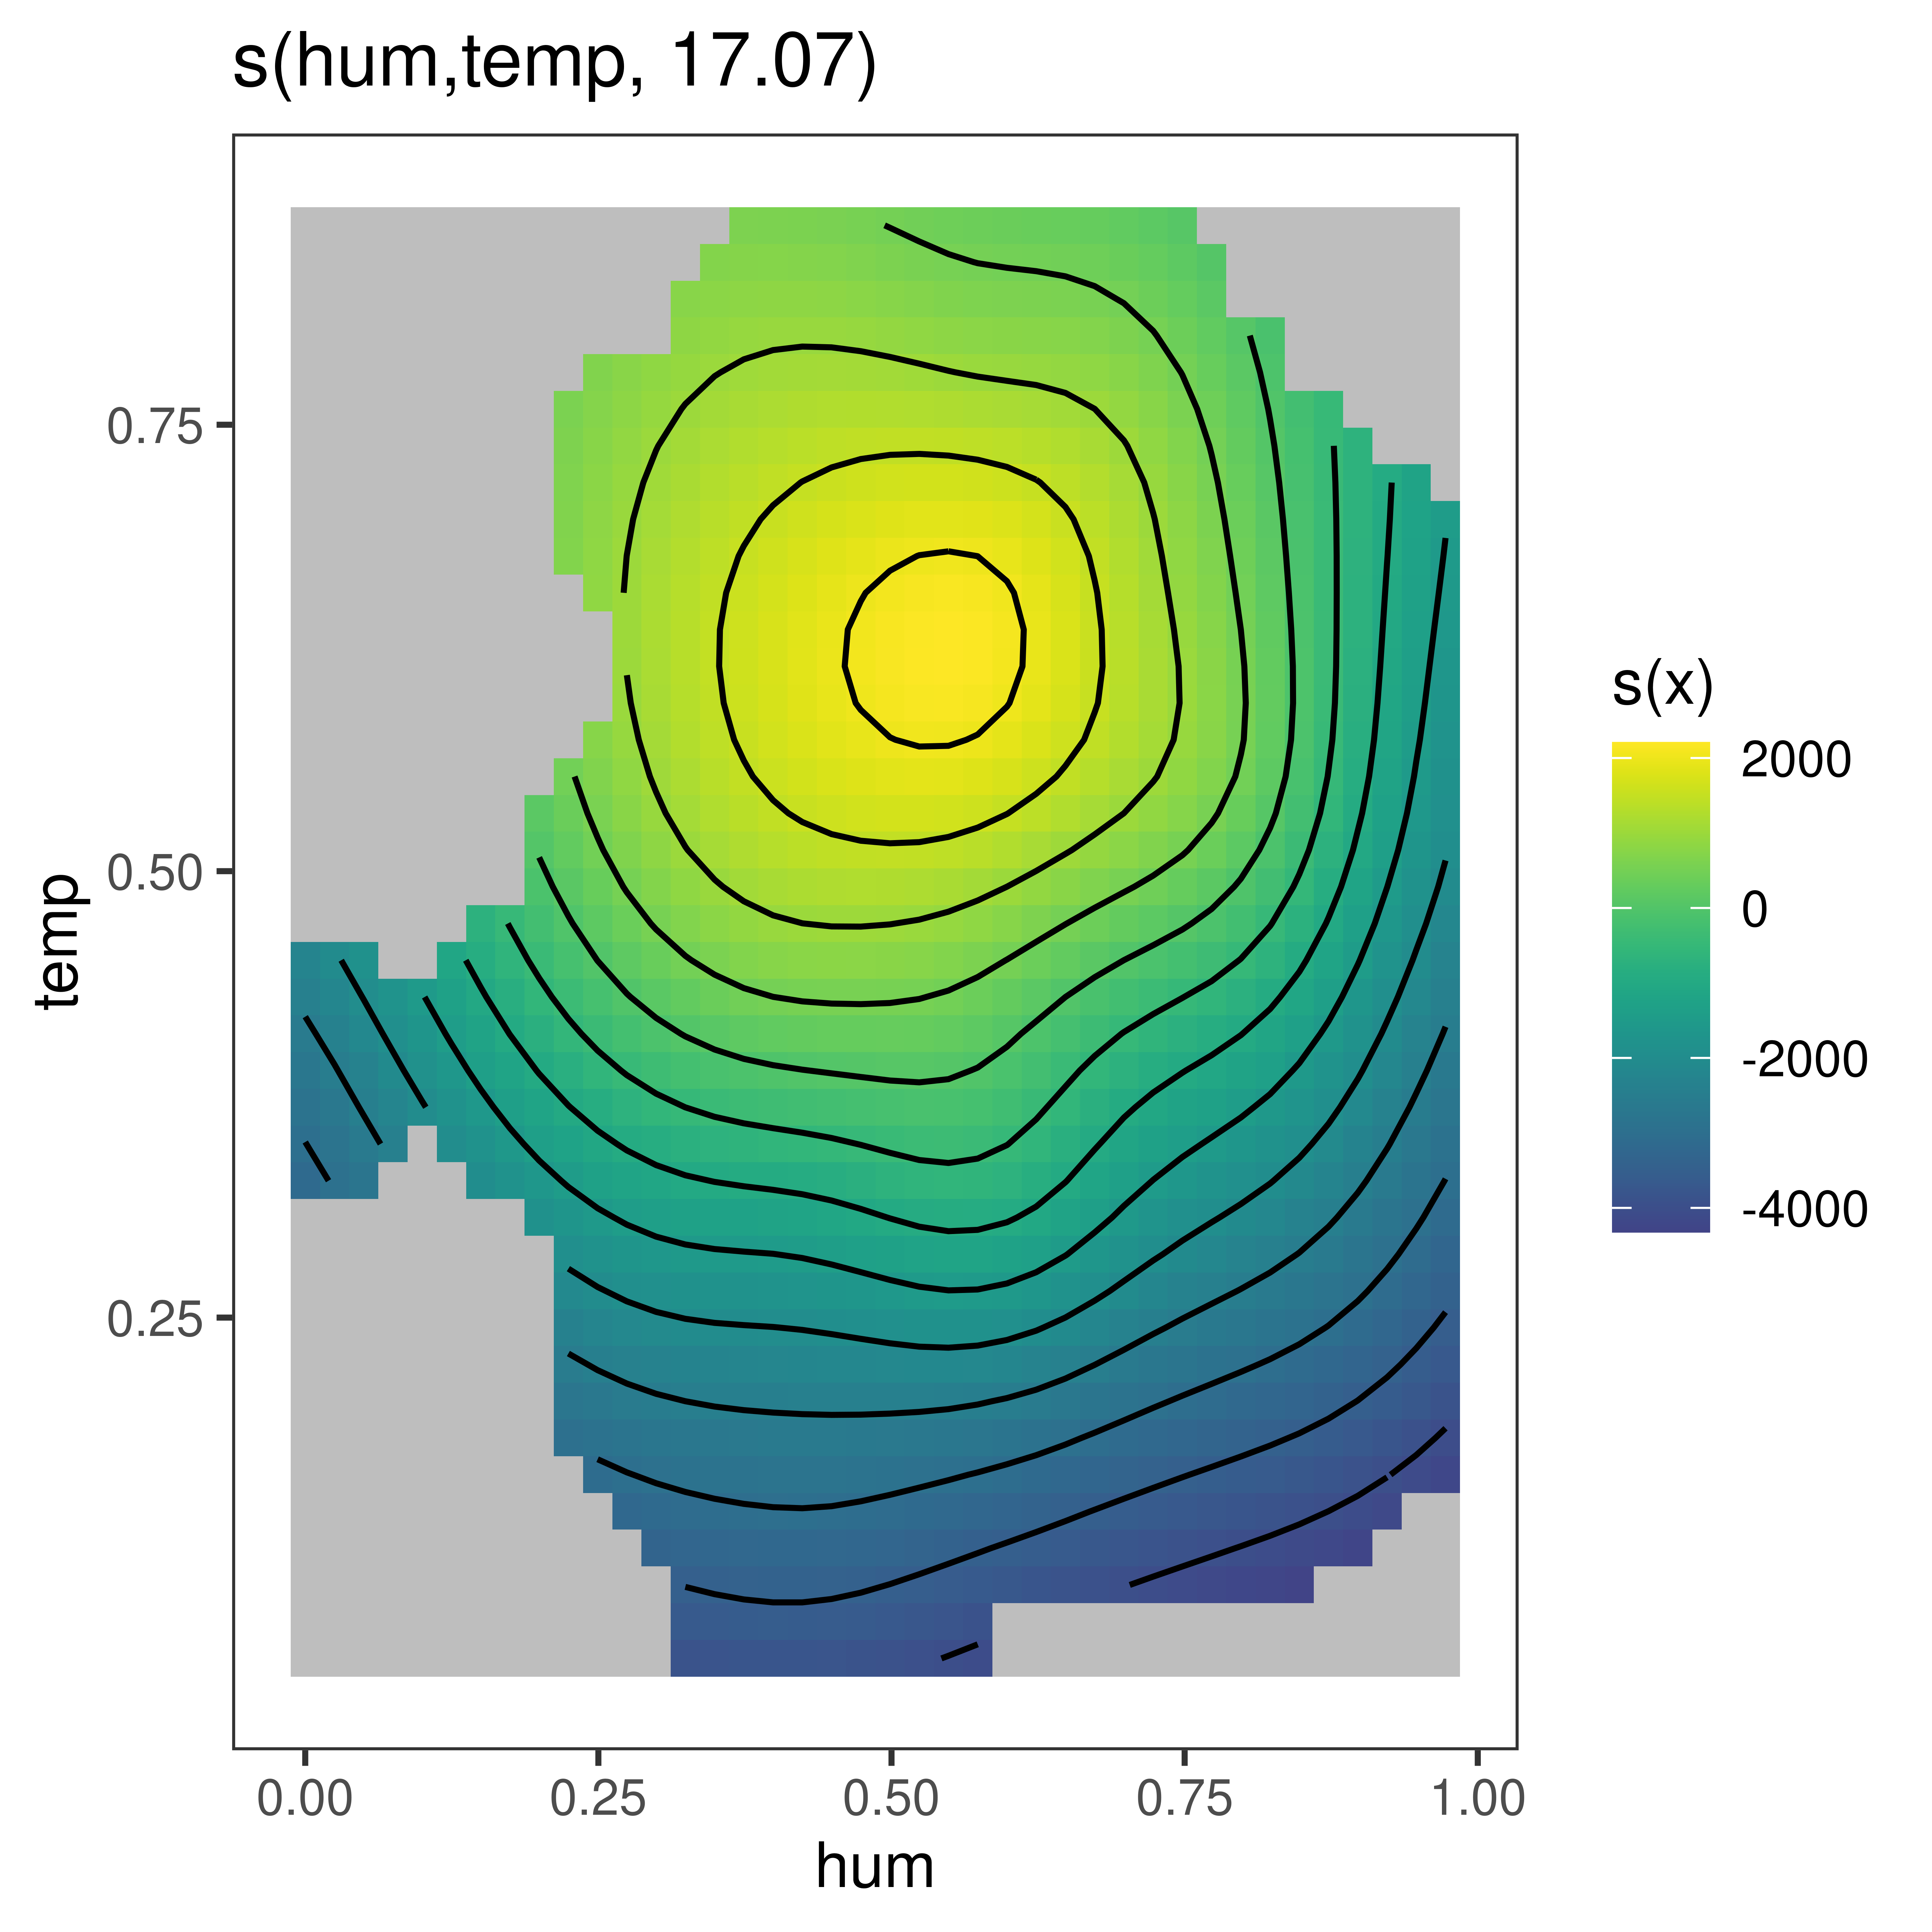
\includegraphics[width = \textwidth]{figure/gam_effect_plot.png}
\end{column}
\end{columns}
\end{frame}


\begin{frame}{Model-Based Boosting}

\begin{itemize}
%\setlength\itemsep{2em}
\item
Boosting iteratively combines weak base learners to create a powerful ensemble model.
\item
Idea: Combine boosting with interpretable base learners (e.g., single feature LM). 
%The resulting ensemble is also interpretable.
\item
Consider two linear base learners $b_j(x, \theta)$ and $b_j(x, \theta^{\star})$ of the same type, but distinct parameter vectors $\theta$ and $\theta^{\star}$. They can be combined in a base learner of the same type:
$$
b_j(x, \theta) + b_j(x, \theta^{\star}) = b_j(x, \theta + \theta^{\star})
$$
\item In each iteration, a selection of base learners is trained on the so-called pseudo residuals. The one with the best fit is added to the previously computed model:
\medskip
\begin{align*}
\widehat{f}^{[1]}(x) &= f_0 + \beta b_3(x_3, \theta^{[1]}) \\
\widehat{f}^{[2]}(x) &= f_0 + \beta b_3(x_3, \theta^{[1]}) + \beta b_3(x_3, \theta^{[2]})\\
\widehat{f}^{[3]}(x) &= f_0 + \beta b_3(x_3, \theta^{[1]}) + \beta b_3(x_3, \theta^{[2]}) + \beta b_1(x_1, \theta^{[3]}) \\
&= f_0 + \beta \left(b_3(x_3, \theta^{[1]} + \theta^{[2]}) + b_1(x_1, \theta^{[3]})\right)
\end{align*}

\item Final model has additive structure (as GAMs), where each component function is interpretable.

\end{itemize}
\end{frame}



% \begin{frame}{Linear Regression}

%     $$y = \beta_0 + \beta_1 x_1 + \beta_2 x_2 + \ldots + \beta_p x_p + \epsilon $$

%     \begin{itemize}
%         \item $y$ target
%         \item $\beta_i$ weight of input feature $x_j$
%         \item $\epsilon$ remaining error
%         \item[$\rightarrow$] model consists of $p+1$ weights $\beta_i$
%         \item Properties and assumptions:
%         \begin{itemize}
%         \item The relationship between the predictor and the mean of $y$ is linear.
%         \item iid observations
%         \item Homoscedasticity (i.e., constant error variance)
%         \end{itemize}
%     \end{itemize}

% \end{frame}


%     Linearity: The relationship between X and the mean of Y is linear.
%     Homoscedasticity: The variance of residual is the same for any value of X.
%     Independence: Observations are independent of each other.
%     Normality: For any fixed value of X, Y is normally distributed.



%------------------------------------------------------------------
%------------------------------------------------------------------

% \begin{frame}{Interpretation of Linear Regression}

%     $$y = \beta_0 + \beta_1 x_1 + \beta_2 x_2 + \ldots + \beta_p x_p + \epsilon $$

%     Let's consider different feature types:
%     \begin{itemize}
%         \item Numerical features: Increase of numerical value will lead to $\beta_i$ times increased output
%         \item Binary feature: Either weight $\beta_i$ is active (1) or not (0).
%         \item Categorical feature: One-hot-encoding of $L-1$ new features for $L$ categories
%         \item Intercept $\beta_0$: reflects expected features values if features were standardised (0-mean, 1-stdev)
%     \end{itemize}

%     Feature importance:
%     \begin{itemize}
%         \item t-statistic by the estimated weight scaled with its standard error\\ (i.e., less certain about the correct value)
%     \end{itemize}
%     $$t_{\beta_i} = \frac{\beta_i}{SE(\beta_i)} $$
% \end{frame}

% %------------------------------------------------------------------
% %------------------------------------------------------------------

% \begin{frame}{Logistic Regression}

%     $$P(y = 1) =\frac{1}{1 + \exp(-( \beta_0 + \beta_1 x_1 + \beta_2 x_2 + \ldots + \beta_p x_p ))} $$

%     \begin{itemize}
%         \item Probabilistic \alert{classification} model
%         \item Typically, we set the threshold to $0.5$ to predict
%         \begin{itemize}
%             \item Class 1 if $P(y=1) > 0.5$
%             \item Class 0 if $P(y=1) \leq 0.5$
%         \end{itemize}
%     \end{itemize}

% \end{frame}

% %------------------------------------------------------------------
% %------------------------------------------------------------------

% \begin{frame}{Interpretation of Logistic Regression}

%     $$\log \left(\frac{P(y = 1)}{P(y=0)}\right) = \beta_0 + \beta_1 x_1 + \beta_2 x_2 + \ldots + \beta_p x_p  $$

%     \begin{itemize}
%         \item weights relate to log odds-ratio
%         \item Again linear in log odds-ratio
%         \item[$\leadsto$] change by one unit changes the odds ratio by a \alert{factor} of $\exp(\beta_i)$.
%         \medskip

%         \item Interpretation for different feature types is the same as for linear regression
%     \end{itemize}

% \end{frame}

% %------------------------------------------------------------------
% %------------------------------------------------------------------

% \begin{frame}{GLM and Interactions}

%     \begin{itemize}
%         \item Linear models are often too restrictive for many applications
%     \end{itemize}

%     \medskip
%     Non-Gaussian outputs via Generalized Linear Models (GLMs):
%     $$g(\mathrm{E}_Y (y\mid x)) = \beta_0 + \beta_1 x_1 + \beta_2 x_2 + \ldots + \beta_p x_p$$
%     \begin{itemize}
%         \item link function $g$ -- can be freely chosen
%         \item exponential family defining $\mathrm{E}_Y$ -- can be freely chosen
%         \item weighted sum $X^\top W$
%     \end{itemize}

%     \medskip

%     Interaction effects via feature engineering:
%     \begin{itemize}
%         \item E.g., feature expansion: $\beta_{x_i,x_j} x_i \cdot x_j$
%     \end{itemize}

% \end{frame}

% %------------------------------------------------------------------
% %------------------------------------------------------------------

% \begin{frame}{Generalized Additive Models (GAMs)}

% Non-Linear relations can be addressed by:
%     \begin{itemize}
%         \item feature transformations (e.g., exp or log)
%         \item Categorization of features (i.e., intervals / buckets of feature values)
%         \item GAMs:
%     \end{itemize}

%     $$g(\mathrm{E}_Y (y\mid x)) = \beta_0 + f_1(x_1) + f_2(x_2) + \ldots + f_p(x_p)$$

%     \begin{itemize}
%         \item instead of $\beta_i x_i$ use flexible functions $f_i(x_i)$ $\leadsto$ splines
%     \end{itemize}

% \end{frame}

% %------------------------------------------------------------------
%------------------------------------------------------------------




\begin{frame}{Model-Based Boosting}
\begin{columns}[T]
\begin{column}{0.55\textwidth}
\scriptsize
\verbatiminput{figure/mboost_output.txt}
\end{column}
\begin{column}{0.45\textwidth}  %%<--- here
  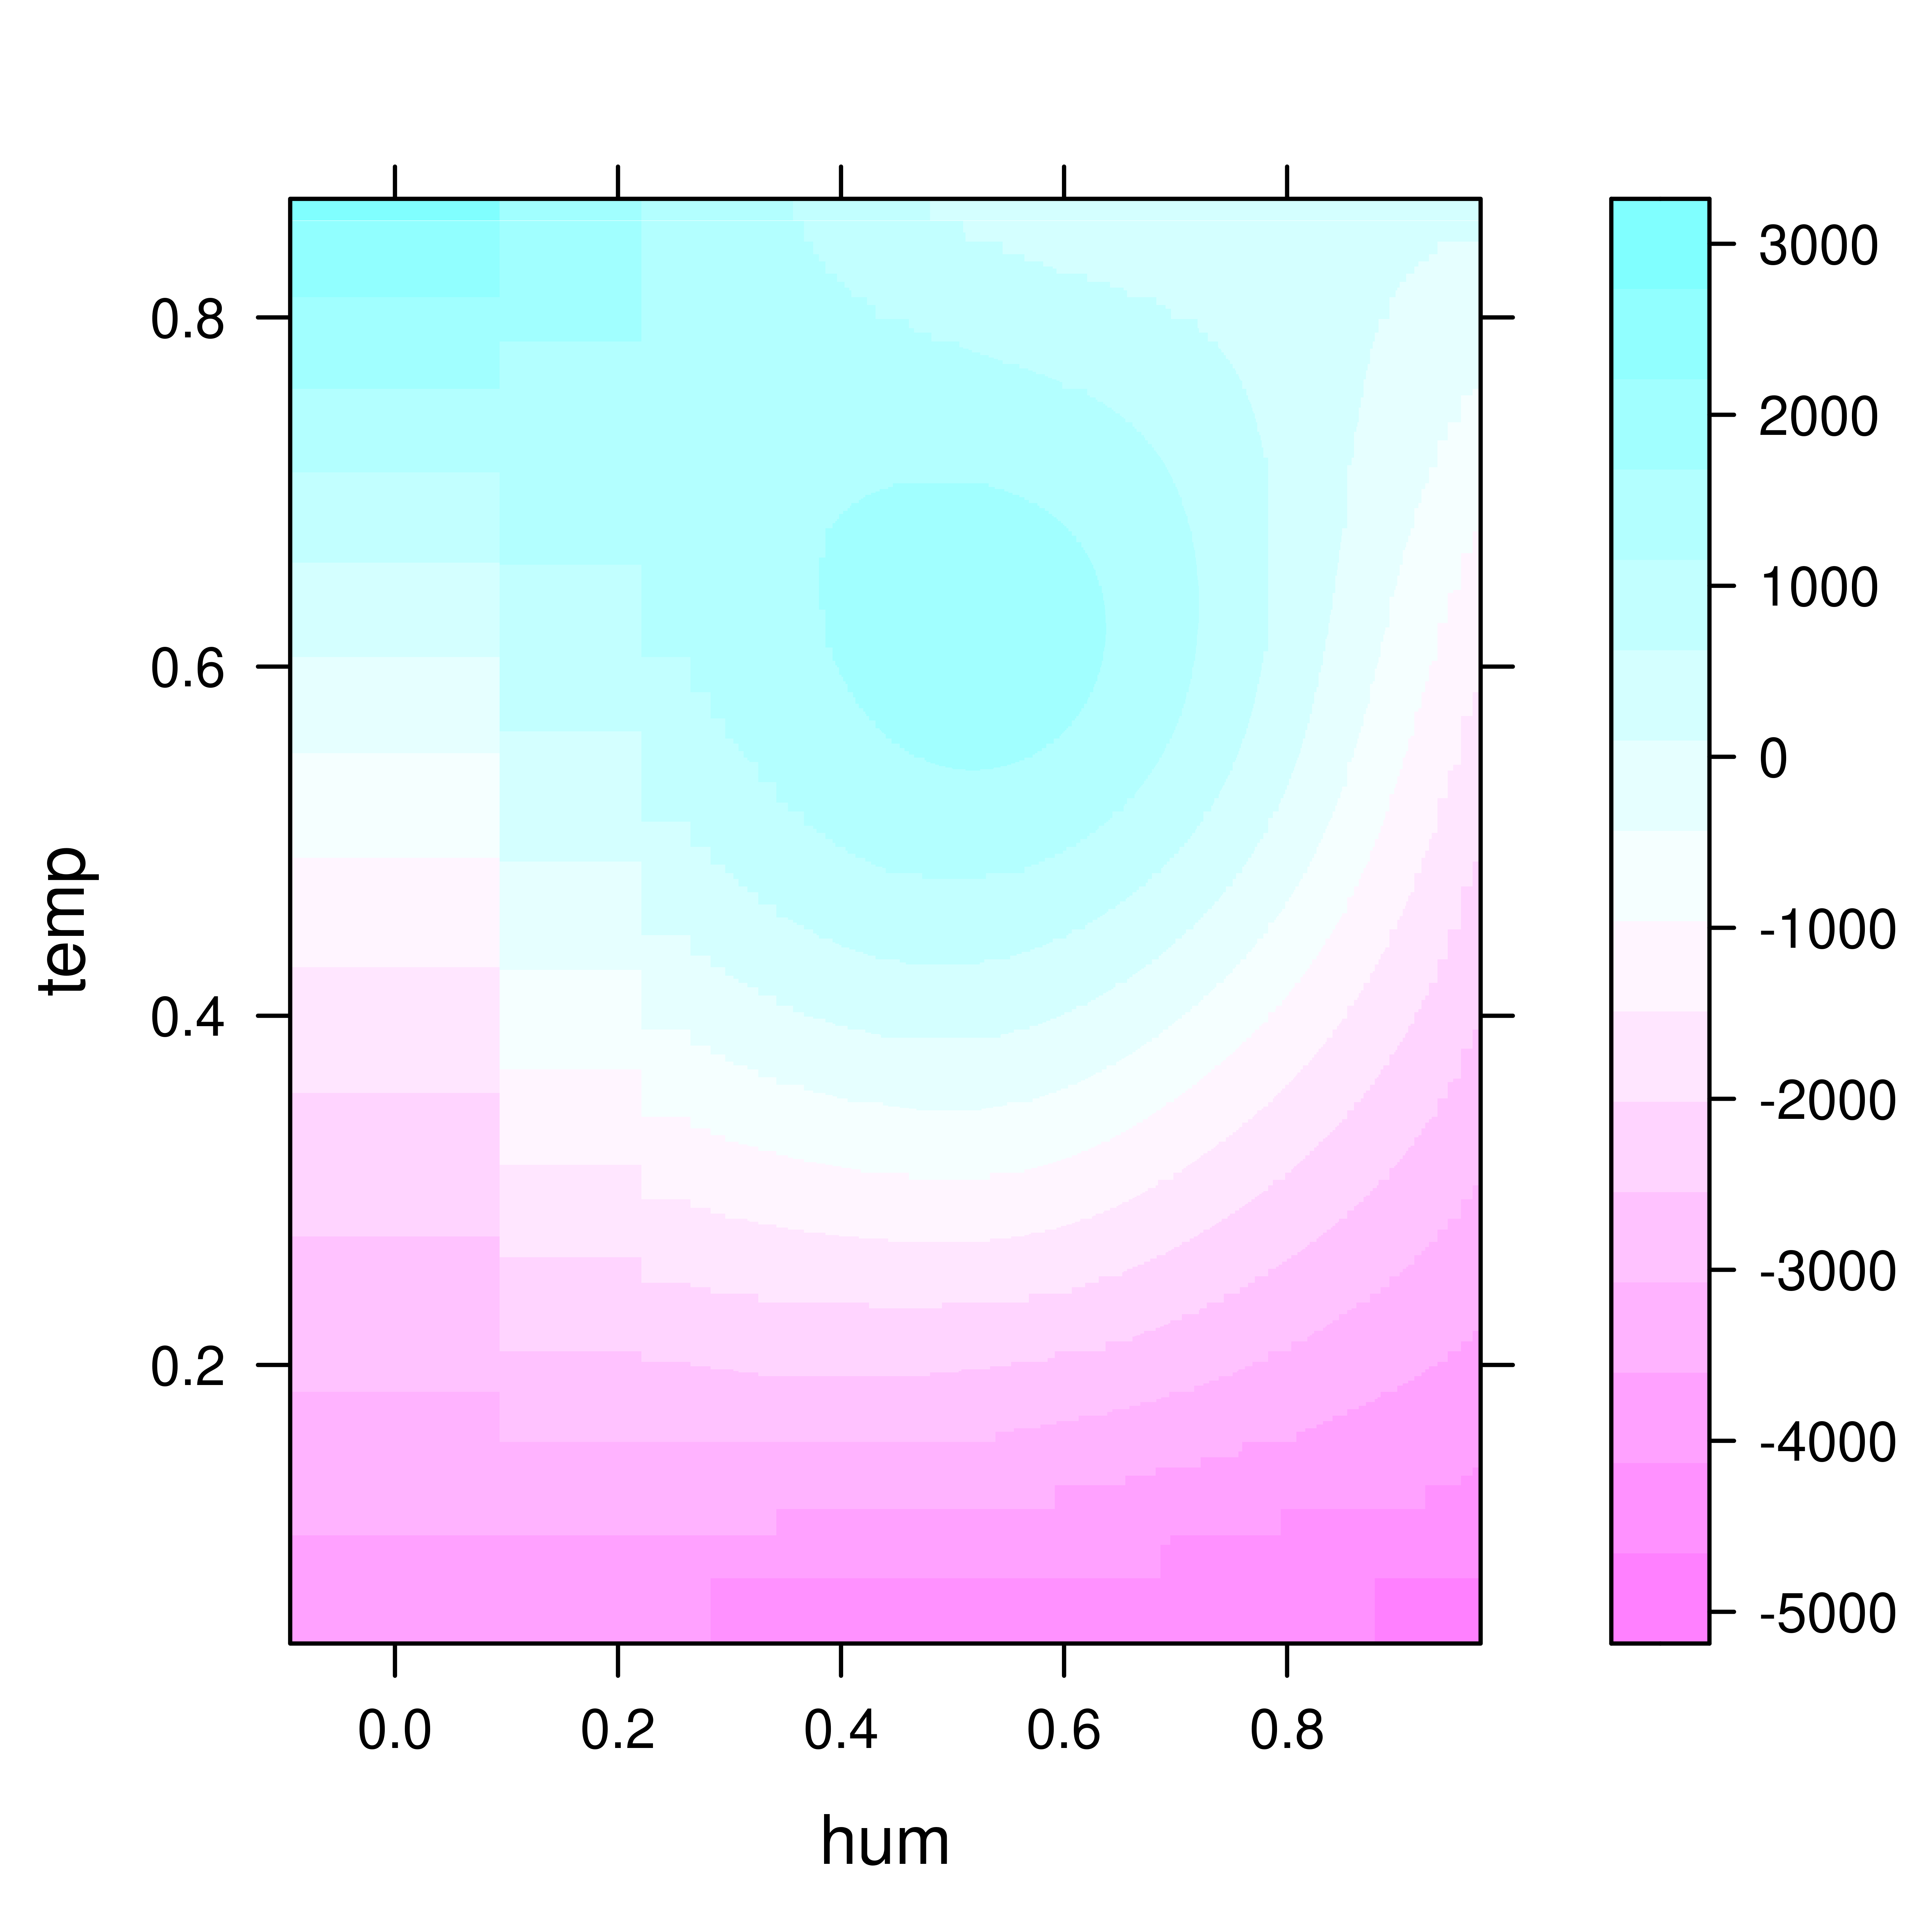
\includegraphics[width = \textwidth]{figure/mboost_effect_plot.png}
\end{column}
\end{columns}
\end{frame}








\begin{frame}{Decision Trees}

\begin{columns}

\begin{column}{0.3\textwidth}

  \begin{tikzpicture}
  \usetikzlibrary{arrows}
    \usetikzlibrary{shapes}
     \tikzset{treenode/.style={draw, circle, font=\small}}
     \tikzset{line/.style={draw, thick}}
     \node [treenode, draw=red] (a0) {$a_0$};
     \node [treenode, below=0.75cm of a0, xshift=-1cm]  (a1) {$a_1$};
     \node [treenode, draw=red, below=0.75cm of a0, xshift=1cm]  (a2) {$a_2$};

     \node [treenode, draw=red, below=0.75cm of a2, xshift=-1cm] (a3) {$a_3$};
     \node [treenode, below=0.75cm of a2, xshift=1cm]  (a4) {$a_4$};

     \node [treenode, below=0.75cm of a3, xshift=-1cm] (a5) {$a_5$};
     \node [treenode, below=0.75cm of a3, xshift=1cm]  (a6) {$a_6$};

     \path [line] (a0.south) -- + (0,-0.4cm) -| (a1.north) node [midway, above] {$x_1<0.3$};
     \path [line] (a0.south) -- +(0,-0.4cm) -|  (a2.north) node [midway, above] {$x_1\geq0.3$};

     \path [line] (a2.south) -- + (0,-0.4cm) -| (a3.north) node [midway, above] {$x_1<0.6$};;
     \path [line] (a2.south) -- +(0,-0.4cm) -|  (a4.north) node [midway, above] {$x_1\geq0.6$};


     \path [line] (a3.south) -- + (0,-0.4cm) -| (a5.north) node [midway, above] {$x_2<0.2$};;
     \path [line] (a3.south) -- +(0,-0.4cm) -|  (a6.north) node [midway, above] {$x_2\geq0.2$};

  \end{tikzpicture}

\end{column}

\begin{column}{0.7\textwidth}

Properties:
\begin{itemize}
    \item able to model non-linear effects
    \item terminal nodes (aka leaf nodes) can have several observations and predicts the mean outcome over these
    \item Applicable to regression and classification
\end{itemize}

Interpretation:
\begin{itemize}
    \item directly by following the tree (i.e., sequence of rules)
    \item Feature importance by (scaled) score of much the splitting criterion was reduced compared to the parent
\end{itemize}

\end{column}

\end{columns}

\end{frame}


\begin{frame}{Decision Trees}

\begin{columns}[T]
  \begin{column}{0.5\textwidth}
     \tiny
     \verbatiminput{figure/rpart_output.txt}
  \end{column}
  \begin{column}{0.5\textwidth}
      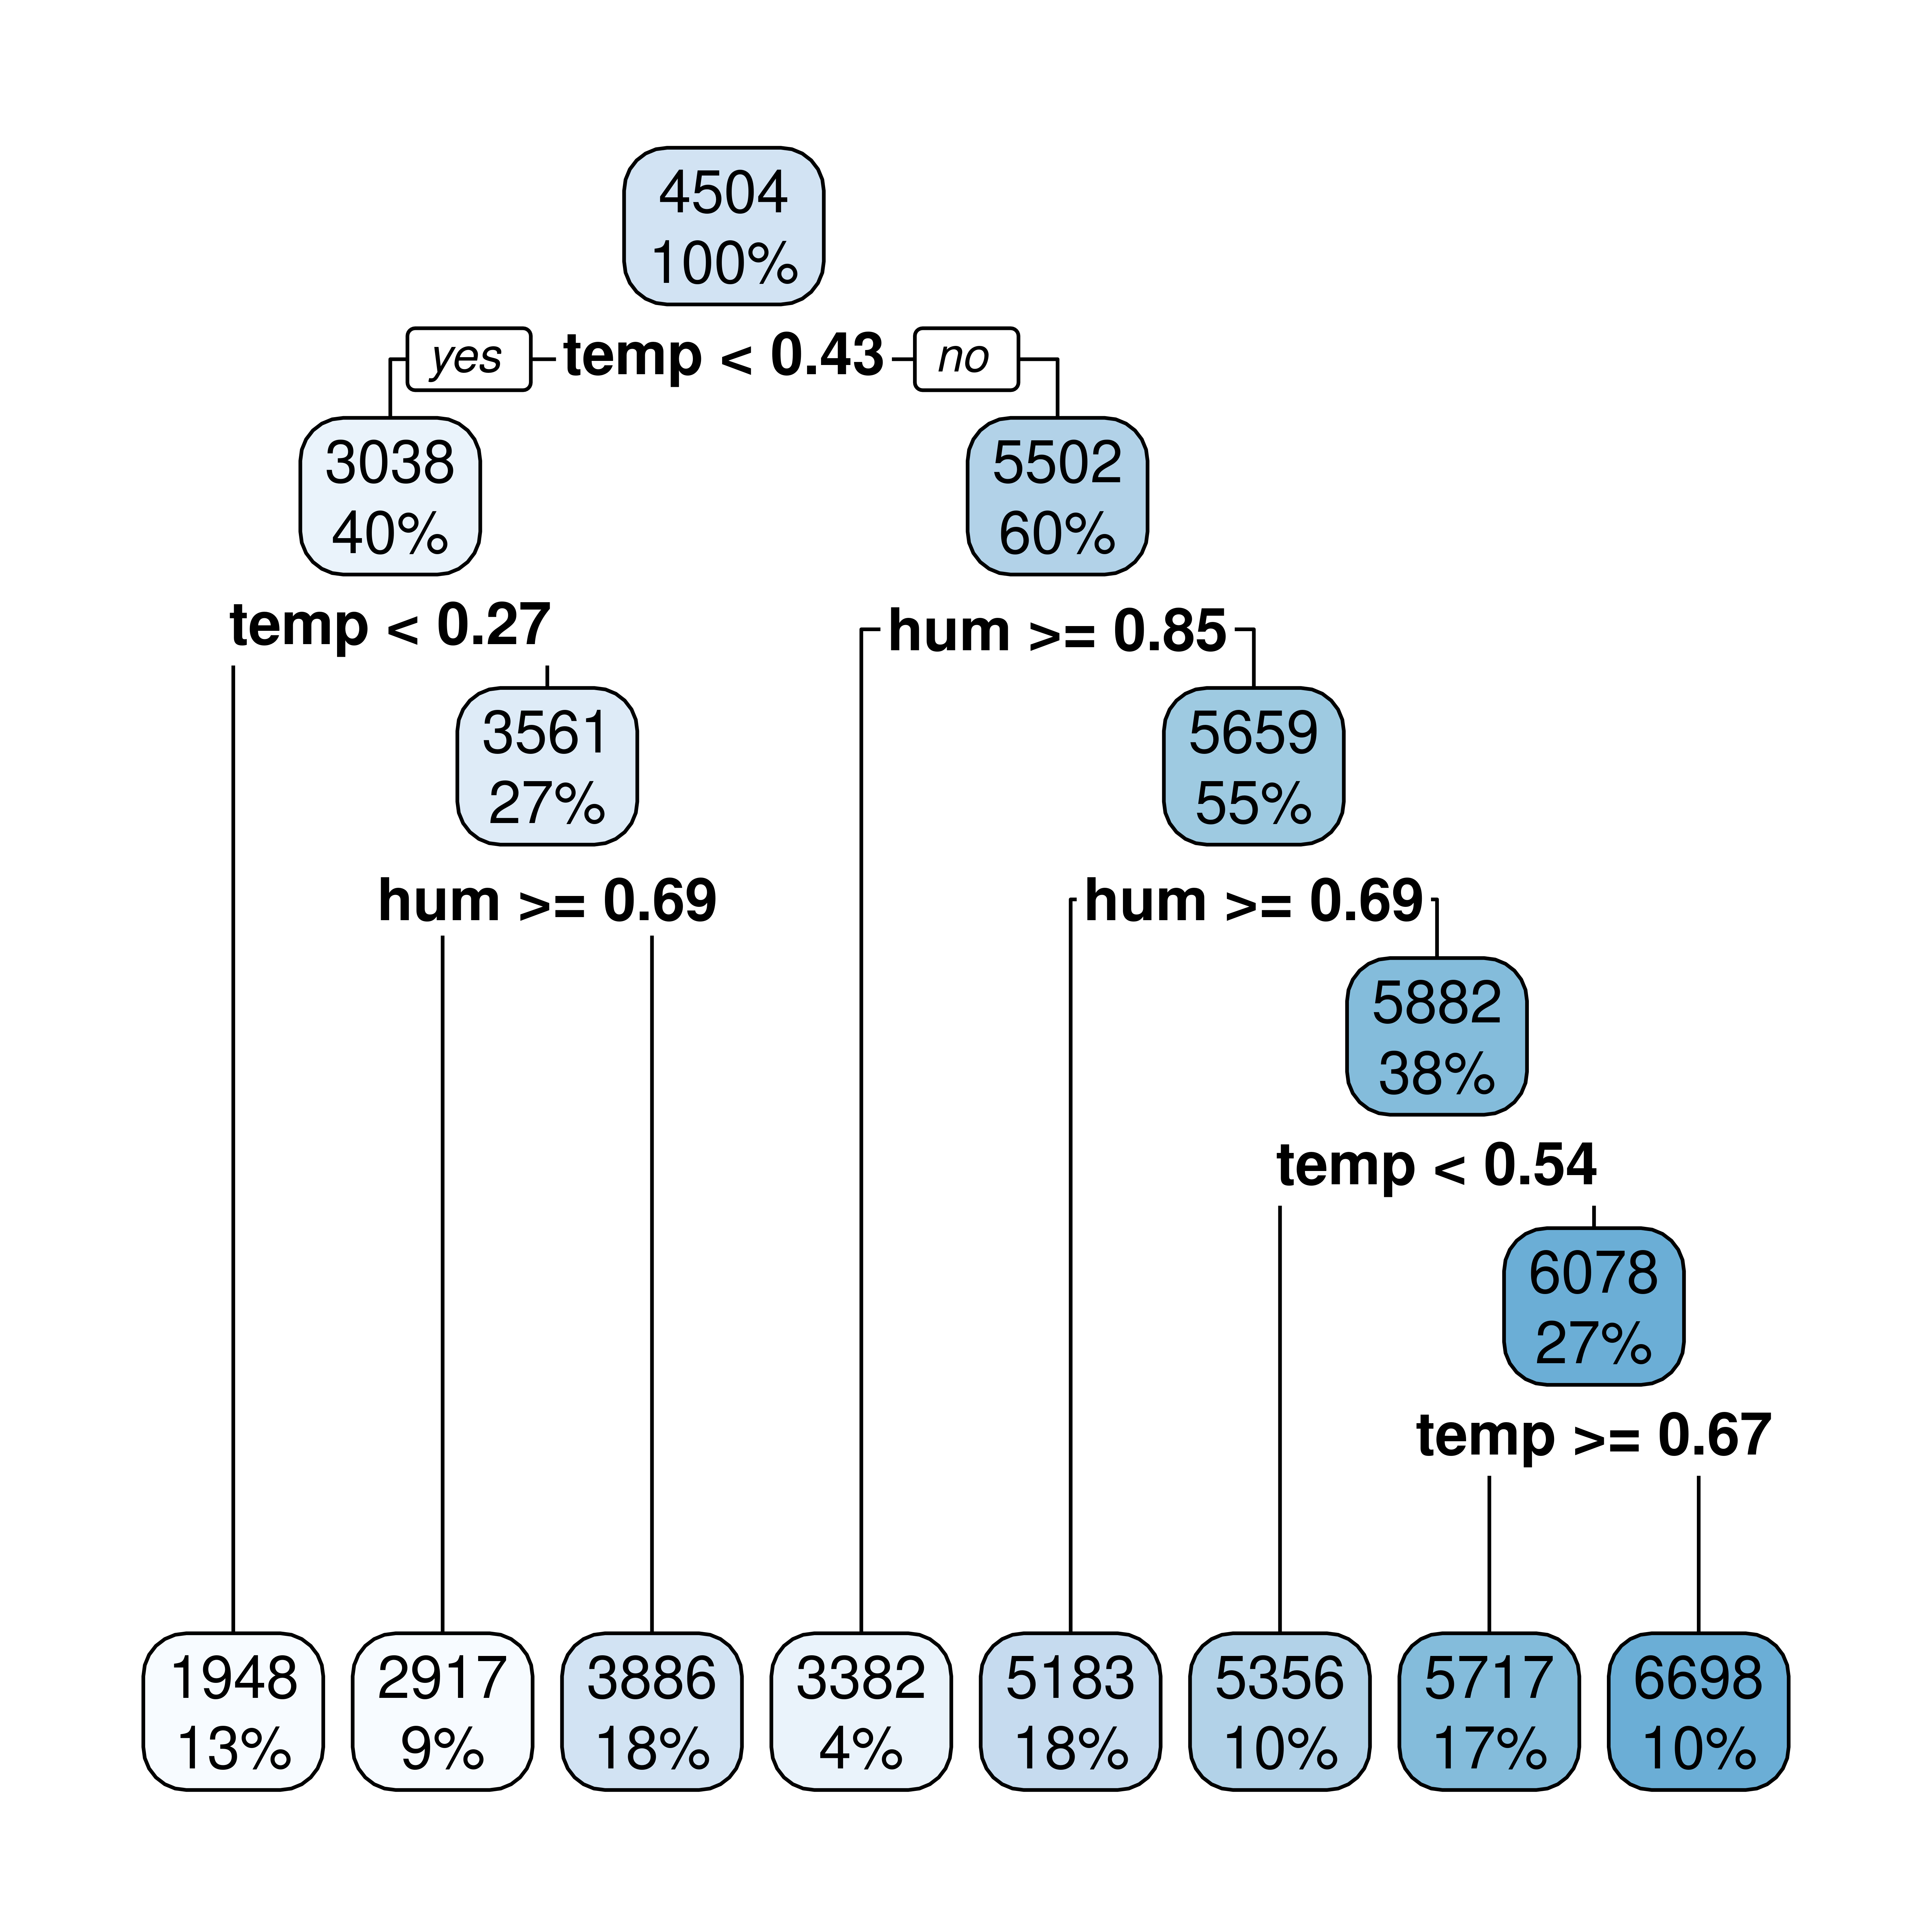
\includegraphics[width = \textwidth]{figure/rpart_plot.png}
  \end{column}
\end{columns}

\end{frame}

%------------------------------------------------------------------
%------------------------------------------------------------------

\begin{frame}{Decision Rules}

\texttt{IF COND$_1$ AND COND$_2$ AND ... THEN value}

\begin{itemize}
    \item \texttt{COND$_i$} can be of the form \texttt{feature <op> value} where \texttt{<op>} can be for example $\{=, <, > \}$
\end{itemize}


\medskip

Properties:
\begin{description}
    \item[Support] Fraction of observations to support appliance of rule
    \item[Accuracy] for predicting the correct class under the condition(s)
\end{description}

$\leadsto$ often trade-off between these two


\medskip

$\leadsto$ many different ways to learn a set of rules (incl. a default rule if none of the rules are met)

\end{frame}



% \begin{frame}{Rule-Based Learning}

% \begin{itemize}
% %\setlength\itemsep{1em}
% \item
% Decision rules follow a general structure: IF conditions are met, THEN make certain prediction.
% \item Although a single decision rule is very intelligibile, a large collection of decision rules might not be. An interpretable rule-based model should therefore be based on as few rules as possible.
% \item Descripte Rule Discovery (DRD) is based on mining databases for frequent item sets, and converting these into a set of decision rules.
% \item For instance, a rule \{mobile phone\} $\Rightarrow$ \{mobile phone case\} indicates that mobile phones and phone cases are bought together frequently.
% \item
% DRD is not suited to create a model that makes predictions on unseen data.
% \item Predictive Rule Learning (PRL) aims to discover a set of rules that cover the entire feature space\footnote[frame]{Fürnkranz J., Kliegr T. (2015) A Brief Overview of Rule Learning. In: Bassiliades N., Gottlob G., Sadri F., Paschke A., Roman D. (eds) Rule Technologies: Foundations, Tools, and Applications. RuleML 2015. Lecture Notes in Computer Science, vol 9202. Springer, Cham.}. There are innumerable rule-based learning algorithms, e.g., decision tree learning, OneR, Sequential Covering, or Bayesian Rule Lists.
% \item Decision tree learning, e.g, classification and regression trees (CART), is the most popular group of rule-based models, as every tree can be represented by a collection of decision rules.
% \item A decision tree recursively partitions the data by optimizing an objective function, e.g., minimizing the data impurity.
% \item A succession of tree splits can be converted to a decision rule by forming a conjunction of successive split criteria.
% \end{itemize}
% \end{frame}


%\item The RuleFit algorithm combines polynomial regression with rule ensembles for automatic interaction detection. In the first stage, a tree ensemble is trained to produce decision rules (where the predictions are discarded and only the splits are utilized), e.g., $x_1 < 0 \land x_2 > 1$. In the second stage, a linear model with main effects is augmented with each decision rule being represented by a single dummy feature.
%\item OneR learns rules from a single feature. OneR is characterized by its simplicity, interpretability and its use as a benchmark.
%\item Sequential covering is a general procedure that iteratively learns rules and removes the data points that are covered by the new rule. This procedure is used by many rule learning algorithms.
%\item Bayesian Rule Lists combine pre-mined frequent patterns into a decision list using Bayesian statistics. Using pre-mined patterns is a common approach used by many rule learning algorithms.
%\end{itemize}


%------------------------------------------------------------------
%------------------------------------------------------------------



%     \begin{frame}{Bike Rentals (Regression)}

%         \begin{itemize}
%             \item Target: number of rented bikes
%             \item Source: bicycle rental company Capital-Bikeshare in Washington D.C.,
%             \item Reference: \footnote{Fanaee-T and Gama. 2014}{https://link.springer.com/article/10.1007/s13748-013-0040-3}
%             \item Exemplary features:
%             \begin{itemize}
%                 \item season: spring, summer, fall or winter.
%                 \item holiday or not.
%                 \item working day or weekend
%                 \item weather situation on that day
%                 \item temperature
%             \end{itemize}
%         \end{itemize}

%     \end{frame}

%     \begin{frame}{Regression on Bike Rentals}

%         \centering
%         \includegraphics[width=0.55\textwidth]{figure/lin_bikesharing.png}

%     \end{frame}

%     \begin{frame}{Decision Tree on Bike Rentals}

%         \centering
%         \includegraphics[width=0.55\textwidth]{figure/dt_bike_sharing.png}

%     \end{frame}

%     \begin{frame}{Risk Factors for Cervical Cancer (Classification)}

%         \begin{itemize}
%             \item Target: patient will get cancer or not?
%             \item Reference: \footnote{Fernandes et al. 2017, \url{https://link.springer.com/chapter/10.1007/978-3-319-58838-4_27}}
%             \item Exemplary features:
%             \begin{itemize}
%                 \item Age in years
%                 \item Number of sexual partners
%                 \item First sexual intercourse (age in years)
%                 \item Number of pregnancies
%                 \item Smoking yes or no
%                 \item Smoking (in years)
%                 \item Hormonal contraceptives yes or no
%                 \item Hormonal contraceptives (in years)
%                 \item Intrauterine device yes or no (IUD)
%             \end{itemize}
%         \end{itemize}

%     \end{frame}

% 	\begin{frame}{Logistic Regression on  Cancer (Classification)}

%         \centering
%         \includegraphics[width=0.55\textwidth]{figure/lin_cancer.png}

%     \end{frame}

% 	\begin{frame}{Decision Tree on  Cancer (Classification)}

%         \centering
%         \includegraphics[width=0.55\textwidth]{figure/dt_cancer.png}
%     \end{frame}

% 	\begin{frame}{Predictive Performance}

%         \begin{itemize}
%             \item Bike Rental (normalized MSE):
%             \begin{itemize}
%                 \item Linear Regression: 0.0276
%                 \item Decision Tree: 0.0328
%                 \item GLM: 0.0244
%             \end{itemize}

%             \medskip
%             \item Cancer (Accuracy)
%             \begin{itemize}
%                 \item Logistic Regression: 0.58
%                 \item Decision Tree: 0.62
%             \end{itemize}

%             \smallskip
%             \item[$\leadsto$] although easy to interpret, not really well-performing
%             \begin{itemize}
%                 \item Boosting: 0.79
%             \end{itemize}
%         \end{itemize}

%     \end{frame}


\endlecture
\end{document}
